% !TEX root = ../main.tex
\chapter{Preliminaries}
\label{chap:preliminaries}

In this chapter I introduce the conceptual foundations and related technologies of my work. Here I discuss the building blocks required to create a static analyzer framework for JavaScript.

\section{JavaScript}
\subsection{ECMAScript 2015}
\subsection{WebAssembly}


\section{Static Analysis}
Even in 1995, the idea of static analysis was over 25 years old: \textquote[\cite{wichmann_industrial_1995}]{The idea  that  computer  software  should be used to analyse source programs rather than compile them, has a history of at least 25 years.}

Source code analysis can be used to discover facts about a particular program. Two basic automated analysis methods exist for source code analysis:
\begin{itemize}[topsep=0pt]
  \item \emph{Static analysis} is performed by reading the source code and analyzing it without evaluating the statements or executing the program.
  \item \emph{Dynamic analysis} is performed by executing the program and evaluating its output for given input sequences.
\end{itemize}

% > The term is usually applied to the analysis performed by an automated tool, with human analysis being called program understanding, program comprehension, or code review. Software inspections and Software walkthroughs are also used in the latter case.
% https://en.wikipedia.org/wiki/Static_program_analysis

While JavaScript is usually not compiled, high-level language source codes are audited at least by the compiler. Thus a specific static analysis should aim to discover unwanted traits of the source in ways a generic compiler could not do, resulting in better code quality. These treats, \emph{bugs} are usually perceptable while running the code. Another way to locate these bugs is to write and run tests, dynamically testing the program.
% \cite[][72]{wichmann_industrial_1995}

The two analysis methods are complementing each other. They discover different subsets of problematic constructions. Information discovered during the static analysis may be used later in the dynamic testing.

% > Static analysis bug-finding tools have evolved over the last several decades from basic syntactic checkers to those that find deep bugs by reasoning about the semantics of code. The goal of the Clang Static Analyzer is to provide a industrial-quality static analysis framework for analyzing C, C++, and Objective-C programs that is freely available, extensible, and has a high quality of implementation.
% http://clang-analyzer.llvm.org/


\subsection{Use Cases}
Static analysis tools employ diverse levels of abstraction. \emph{Formatters} make sure that the source code complies with the style guide. \emph{Linters} check for stylistic and programming errors and warn at suspicious programming constructs. \emph{Formal verification}, on the other hand, utilizes formal mathematical methods to prove or refute statements about the source code and its behavior.

For dynamic languages, it can be used for even more: finding previously undefined property reads, catching invokement of non-functional variables~\cite{jensen_type_2009}, detecting dead code, and so on.

\subsection{Advantages and Disadvantages}

Since static analysis tools deliberately do not evaluate the source code, there are fundamental limitations to what problems they can discover. I consider the following advantages and disadvantages important.


\subsubsection{Advantages}
\paragraph{Input Data Is a By-Product of Compilers}

\paragraph{No Need for Execution}
\begin{itemize}
  \item no need for run environment
  \item no need for mocking, emulating
\end{itemize}

\subsubsection{Disadvantages}
\paragraph{Speed} Static analysis trades CPU time and memory for better code quality. By design it may be multiple orders of magnitude slower than compilation, but its speed depends not only on the underlying data structure and algorithms, but also the level of analysis.
%  > Slower than Compilation
%
%  > Operationally, using static analysis to automatically find deep program bugs is about trading CPU time for the hardening of code. Because of the deep analysis performed by state-of-the-art static analysis tools, static analysis can be much slower than compilation.
%
%  > While the Clang Static Analyzer is being designed to be as fast and light-weight as possible, please do not expect it to be as fast as compiling a program (even with optimizations enabled). Some of the algorithms needed to find bugs require in the worst case exponential time.

However, with a given limitation of granularity, in case of a source code modification, previous results can be reused. There is a possibility that only the modified---and other affected---parts need to be processed again. The incremental approach of static analysis may speed up the process by orders of magnitude~\cite{stein-daniel-bsc}.

\paragraph{False Positives} Static analysis can not prove the correctness of a source code. It rather warn in case there is a possibility of a problem. Thus static analysis tools can introduce false positive warnings and flag code parts as problematic even if they behave correcly.

To reduce the number of false positive warnings, one usually introduces more precise, specified rules and more thorough analysis.

%  > False Positives
%
%  > Static analysis is not perfect. It can falsely flag bugs in a program where the code behaves correctly. Because some code checks require more analysis precision than others, the frequency of false positives can vary widely between different checks. Our long-term goal is to have the analyzer have a low false positive rate for most code on all checks.
%
%  % http://clang-analyzer.llvm.org/

\subsection{Source Code Processing and Analysis}
\label{sect:source-code-processing}
The source code of a program is a sequence of instructions formulated in a programming language as a text. Grammars of formal languages are a set of rules describing what the compiler considers a valid input---how to create valid instructions or a set of instructions from the alphabet of the language \emph{(syntax)}. A source code processing entity (transformer, or hereafter \emph{compiler}) assigns a meaning \emph{(semantics)} and transforms the instruction to another language (generally an intermediate language or bytecode).

What input data the compiler considers useful information depends on the semantics of the language the compiler is built for. Source codes contain a much wider variety of data than a compiler requires for transforming, analyzing the application: comments, function declaration order, indentation, line breaks all help the reader (and writer) of the code, but carry no additional information.

\Cref{fig:processing-the-source-code} shows the general process for processing source code and transforming a stream of characters into a data structure with \emph{meaning}.

\begin{figure}[!ht]
	\centering
	\adjustbox{max width=\textwidth} {
		\begin{tikzpicture}[
			node distance = 1cm,
      label distance = 0.5cm,
			auto,
			]

    \node[stdstage] (SC) {Source Code};
    \node[processor,
          below=of SC,
          label={left:tokenizer}
          ] (TOK) {};
    \node[stdstage, below=of TOK] (TO) {Tokens};
    \node[processor,
          below=of TO,
          label={left:parser}
          ] (PAR) {};
    \node[stdstage, below=of PAR] (AST) {Abstract Syntax Tree};
    \node[processor,
          below=of AST,
          label={left:scope analyzer}
          ] (SA) {};
    \node[stdstage, below=of SA] (ASG) {Abstract Semantic Graph};


    \path (SC) edge[flowedge]  (TOK);
    \path (TOK) edge[flowedge] (TO);
    \path (SC) edge[textedge] node {\emph{tokenization}\\ breaking the stream of source code characters into tokens (words, symbols)} (TO);

    \path (TO) edge[flowedge]  (PAR);
    \path (PAR) edge[flowedge] (AST);
    \path (TO) edge[textedge] node {\emph{parsing}\\ ordering the tokens into a data structure based on grammar rules} (AST);

    \path (AST) edge[flowedge]  (SA);
    \path (SA) edge[flowedge] (ASG);
    \path (AST) edge[textedge] node {\emph{scope analysis}\\ resolving the references in the AST and extending it with derived information into an ASG} (ASG);
		\end{tikzpicture}
	}
	\caption{Processing the source code}
	\label{fig:processing-the-source-code}
\end{figure}

\subsubsection{Lexical Analysis}
A \emph{lexer}, \emph{tokenizer}, or \emph{scanner} forms the first phase of a parsing process. It scans the input character stream and segments them into sequence of groups, tokens, \emph{strings with a ``meaning''}. It also categorizes these groups into various token classes, token types. Processing the raw input into a value (converting the string \code{"2"} into the number $2$) can also happen in this phase. \Cref{fig:tokenization} shows how an expression string can be tokenized.

\begin{figure}[!htb]
  \centering
  \code{foo = 1 / 0}\\[1em]

  \begin{tabular}{c|l}
    Token & Token type\\
    \hline
    \code{foo} & \code{IDENTIFIER (Ident)}\\
    \code{=} & \code{ASSIGN (Punctuator)}\\
    \code{1} & \code{NUMBER (NumericLiteral)}\\
    \code{/} & \code{DIV (Punctuator)}\\
    \code{0} & \code{NUMBER (NumericLiteral)}\\
    \hline
  \end{tabular}

  \caption{Character stream and tokenization result with token type information}
  \label{fig:tokenization}
\end{figure}


\subsubsection{Parser}
A \emph{parser} forms the second phase of a parsing process, using the output token stream of the \emph{lexer}. It takes the input data and builds a hierarchical data structure (a \emph{parse tree} or an \emph{abstract syntax tree}) representing the input. If the input does not comply with the syntax rules, thus an tree can not be built, the source code is syntactically incorrect.

\Cref{fig:sentence-s-expression} shows a sentence and its s-expression representation. S-expressions (for ``symbolic expression'') are a notation for tree-structured nested list, mainly used in Lisp.

\begin{figure}[!htb]
\centering
\code{The quick brown fox jumps over the lazy dog}\\[1em]

\begin{minipage}{3cm}
\begin{verbatim}
(Sentence
  (Word The)
  (Word quick)
  (Word fox)
  (Word jumps)
  (Word over)
  (Word the)
  (Word lazy)
  (Word dog)
)
\end{verbatim}
\end{minipage}
  \caption{A sentence and its s-expression representation}
  \label{fig:sentence-s-expression}
\end{figure}

\paragraph{Abstract Syntax Tree}
An \emph{Abstract Syntax Tree} (AST) is a tree representation of the syntactic structure of the result of a parsing along a grammar. The nodes of the tree denote a construct occuring in the input, while the edges represent the connection between these nodes based on the grammar rules.

As mentioned in~\cref{sect:source-code-processing}, source code contains much more detail (e.g., indentation, whitespace, comments) than is required and restrained during the parsing process. Thus this representation is a digested, \emph{abstract} syntax tree. It may be transformed based on transformation rules and source code can be generated from ASTs. Without restraining the layout information and reusing it during the code generation, the resulting text can show differences in indents, whitespaces and expression formulation compared to the initial source code.

\Cref{fig:ast-asg-example} shows an example AST (in black), where a one-statement JavaScript file is parsed. The content of the file was only \code{var foo = 1 / 0;}.

\subsubsection{Scope Analyzer}
A \emph{scope analyzer} or \emph{context analyzer} produces a data structure that represents the scoping information of a program, probably extending the information available from an AST or an ASG. An element representing a scope in this data structure may contain, inter alia, metadata about the scope itself, the AST node related to the scope, available assets (variables, functions, etc.) in that scope.~\cite{shift-scope}

\paragraph{Abstract Semantic Graph}
As its name implies, an \emph{Abstract Semantic Graph} (ASG), although sounding alike, differs from an Abstract Syntax Tree. (1) ASGs are graphs, and (2) express more than the syntactic information; ASGs carry semantic information expressed with additional edges. These edges can not exist in an AST, as they are non-tree edges (cross-edges). For example they may connect variable references to their declarations.~\cite{raghavan_dex:_2004}

An ASG is a graph representation of a parse result; the nodes represent subterms of an expression. Shared subterms can occur, having more than one node linked to the same, common subterm. Compilers generally work on ASGs internally, since not only the syntactical, but the behavioral information are also represented in them.

% An abstract semantic graph is typically constructed from an abstract syntax tree by a process of enrichment and abstraction. The enrichment can for example be the addition of back-pointers, edges from an identifier node (where a variable is being used) to a node representing the declaration of that variable. The abstraction can entail the removal of details which are relevant only in parsing, not for semantics.
% https://en.wikipedia.org/wiki/Abstract_semantic_graph

\Cref{fig:ast-asg-example} shows the difference between an AST and an ASG (in turquoise).

\begin{figure}[!htb]
	\centering
	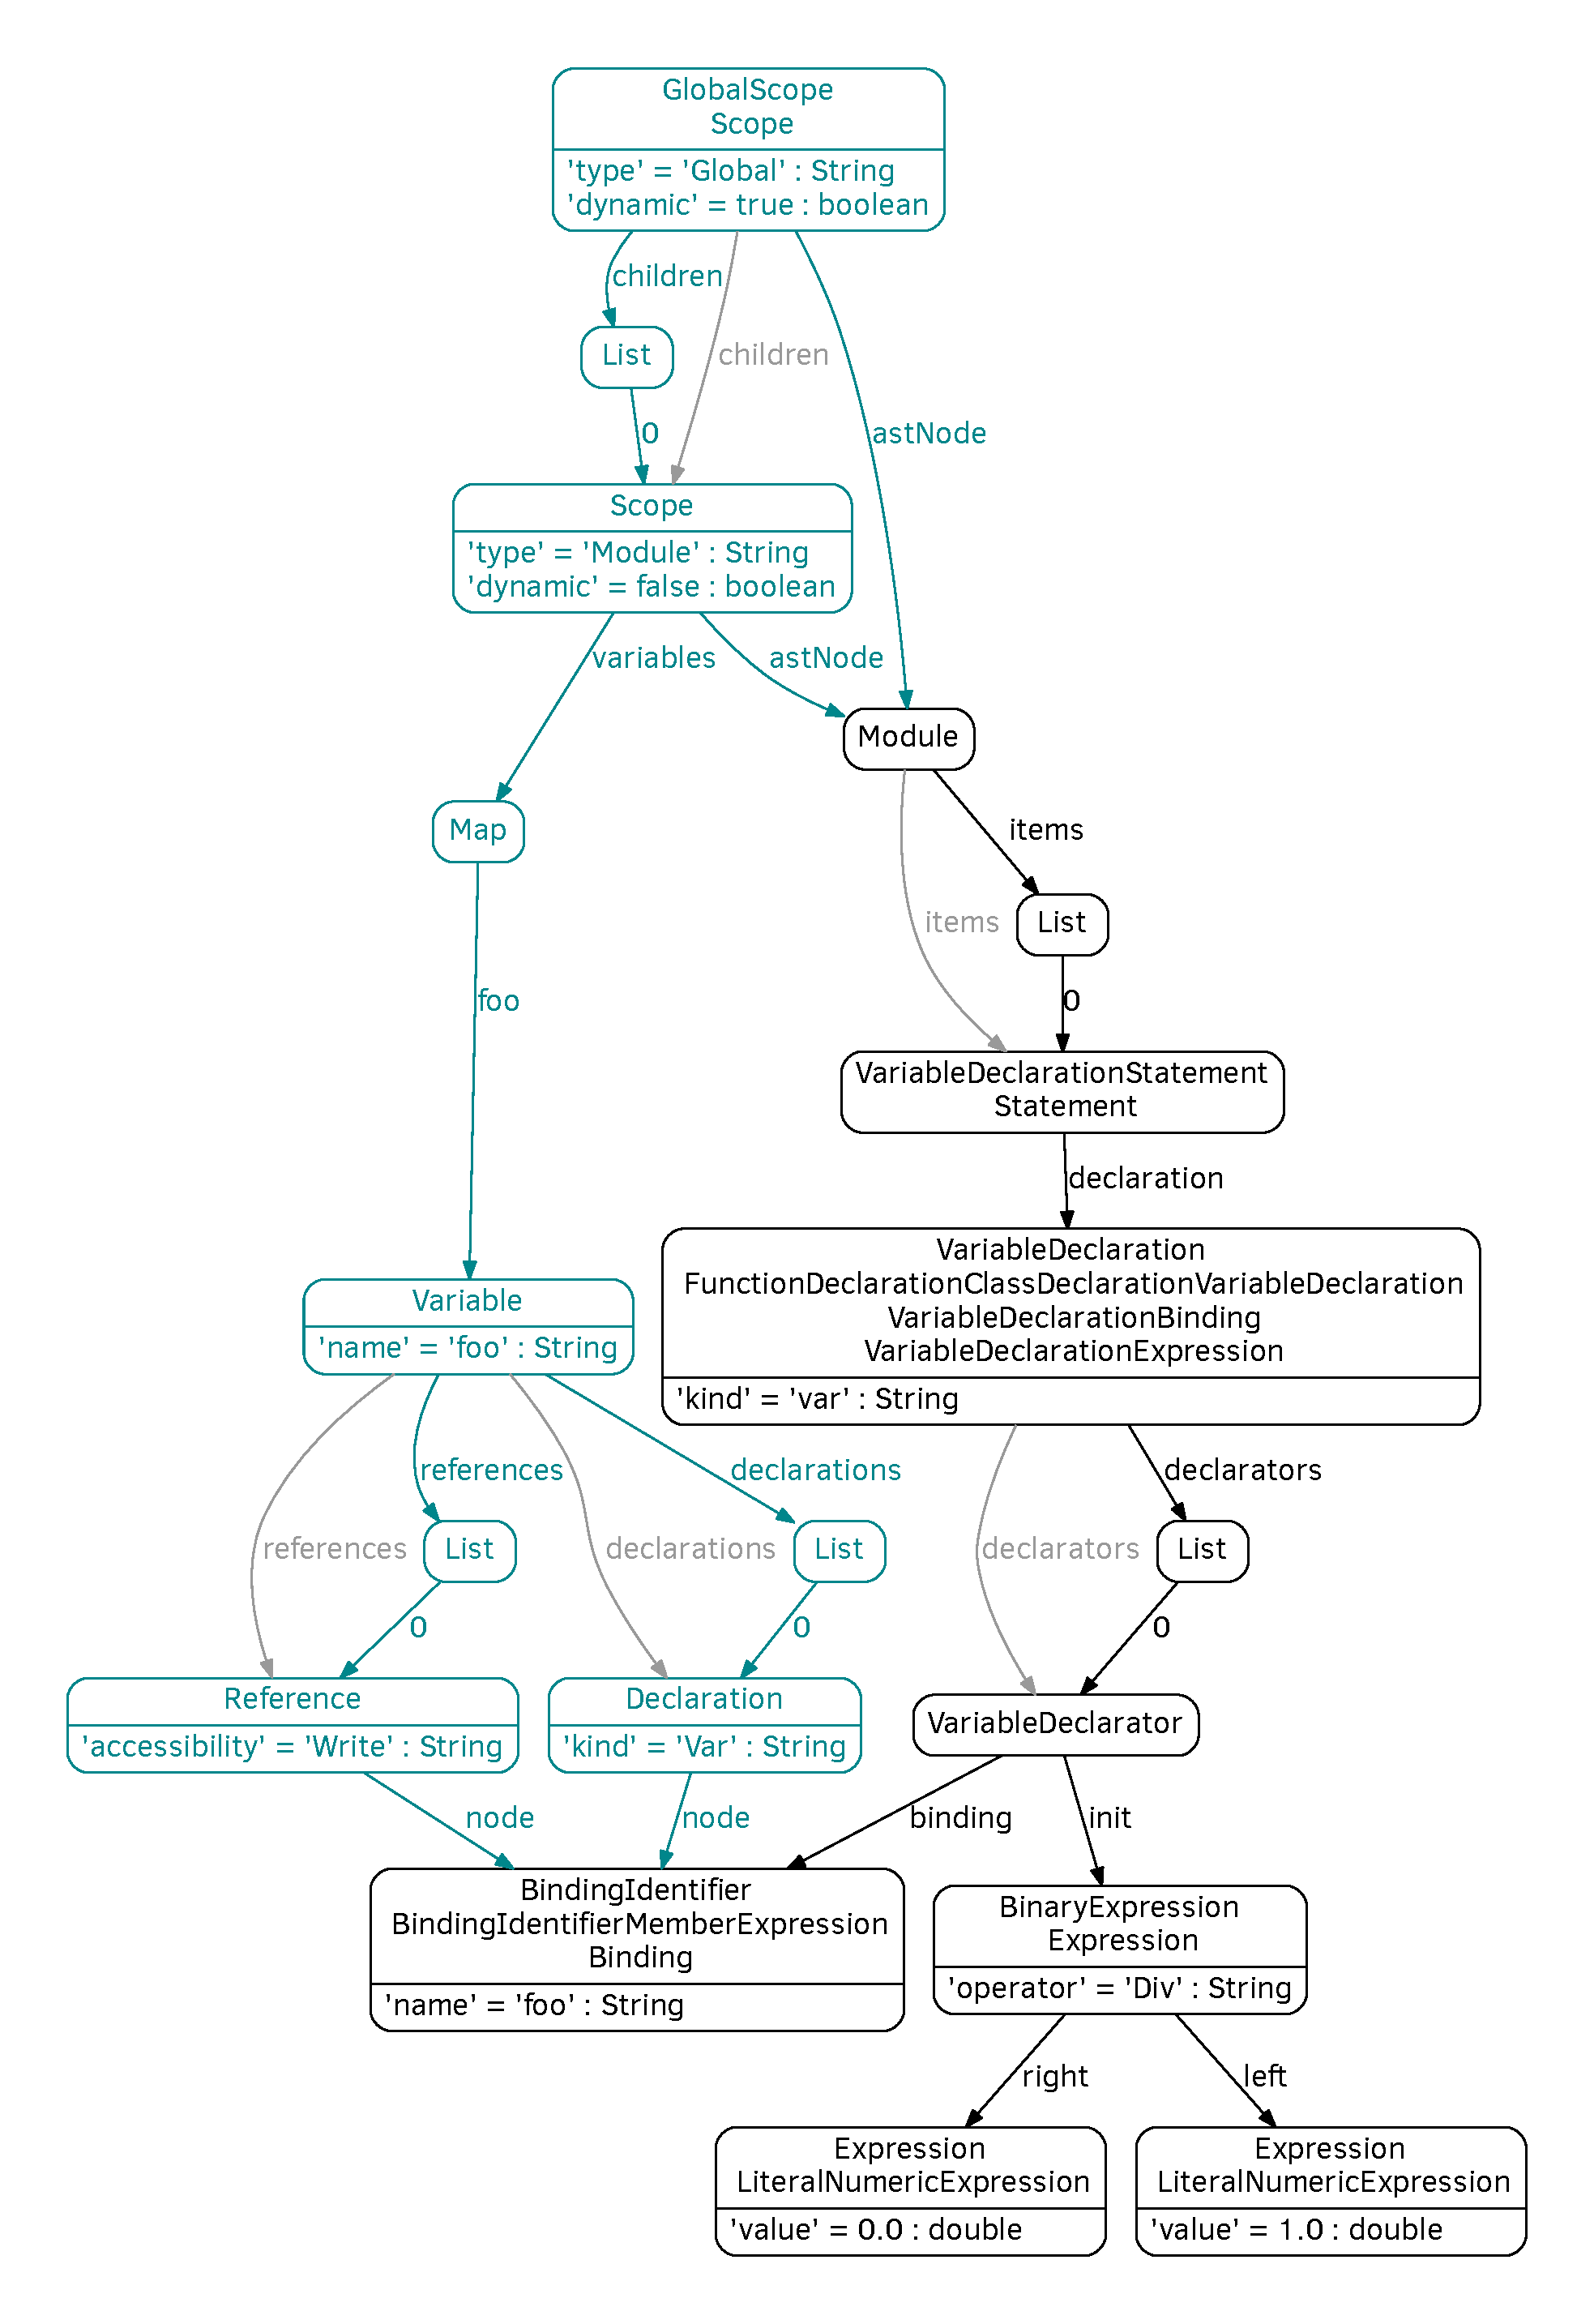
\includegraphics[height=\textheight, trim=1cm 1cm 1cm 1cm,clip]{include/figures/AST-ASG}
	\caption{AST (in black) with additional edges (ASG, in turquoise) and derived helper edges (in gray).}
	\label{fig:ast-asg-example}
\end{figure}

\FloatBarrier

\section{Type Inference}

Type inference refers to the deduction of the data types of expressions, statements during static analysis.

> Type inference refers to the automatic deduction of the data type of an expression in a programming language. If some, but not all, type annotations are already present it is referred to as type reconstruction[citation needed]. The reverse operation of type inference is called type erasure.

> It is a feature present in some strongly statically typed languages. It is often characteristic of functional programming languages in general. Some languages that include type inference are Nim, ML, OCaml, F\#, Haskell, Scala, Go, D, Clean, Opa, Rust, Swift, Visual Basic (starting with version 9.0), C\# (starting with version 3.0) and C++11. The ability to infer types automatically makes many programming tasks easier, leaving the programmer free to omit type annotations while still permitting type checking.

% https://en.wikipedia.org/wiki/Type_inference

\subsection{Typed JavaScript Derivations}

\subsection{Analysis of JavaScript Source Codes}
There are several static analysis frameworks and solutions available for JavaScript. I introduce and compare them in detail in \cref{sect:javascript-parsers} (JavaScript parsers) and \cref{sect:javascript-type-inferencers} (JavaScript type inferencing solutions).


\section{Handling Large Interconnected Data}
The progress of computer parts -- the ever increasing amount of processing power, and memory and storage speed and sizes -- and the alike growth of data to be stored and processed during the last more than fifty years yielded various solutions.

Based on historic evolution, these solutions can be categorized in three main categories:
\begin{itemize}[topsep=0pt]
  \item \emph{Navigational} database management systems (DBMS) were mainly used in the era of magnetic tape based storages, in which the \emph{records} contained references to other records allowing the system to fast-forward, \emph{navigate} there and load additional data.

  \item \emph{Relational} DBMSs organizes data in a \emph{relational model}~\cite{codd}, where one or more \emph{relations} contain unique entries (\emph{records} or \emph{tuples}).

  Relational databases leverage precise mathematical background (see \emph{relational algebra} and \emph{relational calculus}), have diverse implementations, mature tooling, and data access security by authentication and authorization. There are also disadvantages; due to their data structure, relational databases may have scalability and performance issues. They are also typically optimized for transactional processing and not data analysis (there are exceptions, see \emph{data warehouses}).

  \item \emph{Post-relational} databases is a vague collective name for every database system that abandons the strictness and burden of the relational data model and the Structured Query Language (SQL).

  Since the turn of the millennium, the struggle with storing and processing huge amounts of data using relational technologies spawned a diverse palette of new database management systems using simpler, more scalable data models. These systems are consequently called \emph{non SQL}, NoSQL databases, and are increasingly used in real-time and big data applications.

  NoSQL systems are a heterogeneous set of systems, with very different approaches. Categories of these systems based on their data models include, but are not limited to: \emph{key-value stores}, \emph{wide column stores}, \emph{document stores}, \emph{graph DBMSs}, \emph{RDF stores}.
\end{itemize}

Since my approach is based on graph databases, in this section I introduce the concept of graph databases, and graph pattern matching. I also introduce several graph database implementations and systematically compare them in order to select the appropriate technology for the approach.


\subsection{On Graph Computing}
Graphs are well-known and in computer science widely used mathematical concept, which has been around for many decades. Numerous graph technologies have evolved, each with their advantages and disadvantages. From graphs themselves to physical and virtual worlds, many scenarios can be represented as graphs and stored in graph databases with their respective data model. This section loosely follows~\cite{scm, On_Graph_Computing}.

\begin{figure}[!ht]
	\centering
	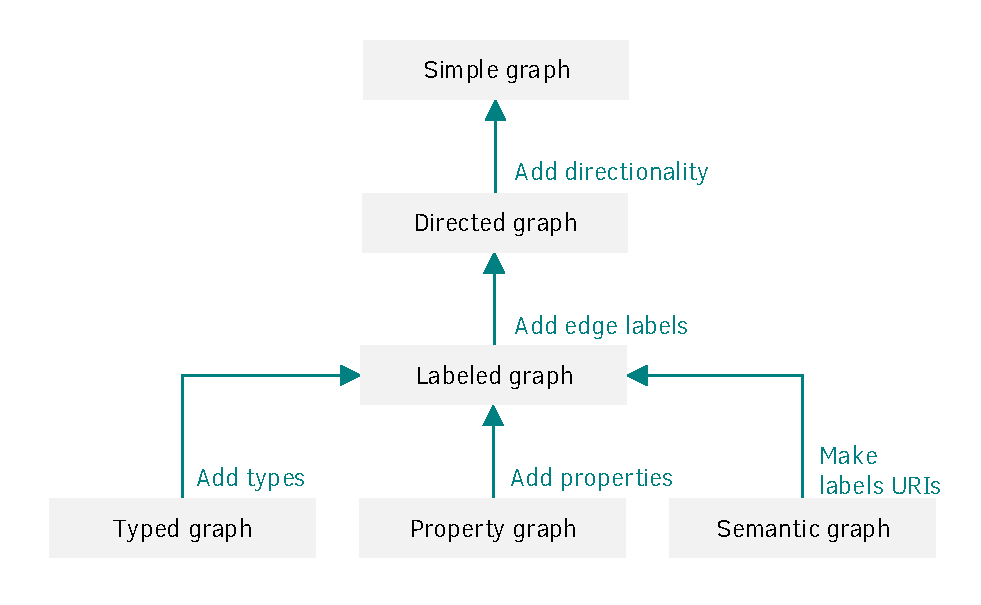
\includegraphics[width=0.8\textwidth]{include/figures/graph-classes}
	\caption{Graph data models~(based on~\cite{DBLP:journals/corr/abs-1006-2361}).}
	\label{fig:graph-classes}
\end{figure}

The most basic graph model is the \emph{simple graph}, formally defined as $G = (V, E)$, where $V$ is the set of vertices and $E \subseteq V \times V$ is the set of edges. Simple graphs are sometimes referred as textbook-style graphs because they are an integral part of academic literature. Simple graphs are useful for modeling homogeneous systems and have plenty of algorithms for processing.

Simple graphs can be extended in several different ways (see \cref{fig:graph-classes}). To describe the connections in more detail, one may add directionality to edges (\emph{directed graph}). To allow different connections, one may label the edges (\emph{labeled graph}).

\emph{Typed graphs} introduce types for vertices. \emph{Property graphs} (sometimes called \emph{attributed graphs}) add even more possibilities by introducing properties. Each graph element, both vertices and edges can be described with a collection of properties. The properties are key--value pairs, e.g.\ \texttt{type = `Person'}, \texttt{name = `John'}, \texttt{age = 34}. \emph{Semantic graphs} use Uniform Resource Identifiers (URIs) instead of labels, otherwise they have similar expressive power as labeled graphs.

My approach utilizes typed (labeled) property graphs.

\subsubsection{Graph Computing Technologies}
The practice of data storage and processing is encumbered with space and time trade-off. This trade-off is also present in various graph computing technologies. This section discusses the categorization of these technologies and mentions a few technologies of which the most popular ones are detailed in~\cref{sect:graph-databases}.

The landscape of graph storing and processing solutions is populated and diverse (see~\cite{zhang_-memory_2015}). The basic categorization is the following. Graph computing technologies can be divided into two groups: on-line, real-time; and global analyzing, batch-processing graph databases. The former can be divided into in-memory, and disk-resilient databases.

\paragraph{In-Memory Graph Toolkits}
The challenge of big data problems shed light on that the existing disk-based systems can not offer timely response due to the latency of hard disks. The role of storage shifted from the hard drive to the memory of the system. In-memory graph databases are constrained to graphs that fit into the main memory. Thus these systems are single-user systems that are oriented towards low-latency graph analysis.

The locality of data allows the usage of rich algorithm libraries and the choice of the adequate graph representation with respective space-time trade-off. The constraint of space allows large graphs (with millions of edges) to be stored and processed, but this is not sufficient in all cases.

Example in-memory graph toolkits: \emph{Apache Giraph}, \emph{Microsoft Graph Engine} (formerly \emph{Trinity}), \emph{Apache Spark GraphX}, \emph{WhiteDB}.

\paragraph{Disk-Resilient, Real-Time Graph Databases}
\paragraph{Batch-Processing Graph Frameworks}

\subsection{Evaluating Queries on a Data Structure}
Numerous strategies exist for defining and executing queries over data structures. They can be defined in an imperative manner with programming languages like a navigation described in \emph{Gremlin} over a graph database or using a data access interface such as the Eclipse Modeling Framework. Declarative solutions also exist, where the query plan is calculated from the query formalized in a declarative language (like frameworks \emph{SQL}, \emph{SPARQL}, \emph{Cypher}) and execution is performed by a query framework (such as \emph{4store}, \emph{Neo4j}). I base my approach on pattern matching, one of the declarative querying solutions, supplemented by imperative logic.

\subsubsection{Graph Pattern Matching}
\textquote[\cite{csmr}]{Graph patterns are a declarative, graph-like formalism representing a condition (or constraint) to be matched against instance model graphs. The formalism is useful for various purposes in model-driven development, such as defining model transformation rules or defining general purpose model queries including model validation constraints. A graph pattern consists of structural constraints prescribing the interconnection between nodes and edges of a given type.

A match of a pattern is a tuple of pattern parameters that fulfill all the following conditions:
\begin{enumerate}[topsep=0pt]
	\item have the same structure as the pattern,
	\item satisfy all structural and attribute constraints,
	\item and does not satisfy any negative application condition (NAC) describing cases when the original pattern does not hold.
\end{enumerate}}


\subsection{Graph Databases}
\label{sect:graph-databases}
Since my thesis work is based on graph-based data handling, it is essential to use a technique that is suitable. In this case suitable is better described as being fast, flexible, versatile, easy to use and deploy. In this section I go over some of the most promising candidates and justify why I have chosen Neo4j as the foundation of my approach.

\subsubsection{Neo4j}
Neo4j is one of the most popular and most mature NoSQL graph databases developed by \emph{Neo Technology}. It is open-source, well-documented and steadily-developed. Neo4j is available in two editions: a free \emph{Community Edition} and a paid \emph{Enterprise Edition}.~\cite{neo4j}

\paragraph{Architecture}
Since Neo4j was written in Java (and Scala), it can be used to start a new project quick and easy. In respect of connection, it can be deployed two ways: in \emph{server mode} the database is started separately and listens for queries on its HTTP REST and Bolt interface; where in \emph{embedded mode} it runs in the same JVM as the only client application.

\paragraph{Data Model}
The graph model in Neo4j, \code{Neo4jGraph} is an implementation of the \emph{TinkerPop} graph computing framework's \emph{Blueprints} property graph data model. More precisely it is a labeled property graph, since the relations are labeled and the nodes can also hold multiple labels; the nodes and relations can both hold properties.

Unfortunately the relations are only binary, ternary (and n-ary $n>2$) relations can only be stored with an introduced indirection, a connection node connecting every node in the relation.

\paragraph{Sharding}
Although the \emph{Enterprise Edition} of Neo4j has a high availability solution and supports clustered replication and cache sharding, it does not support sharded data storage over a cluster of devices. This results in the advantage of low latency (clustering provides scale out capabilities for read), the ability to handle transactions and having ACID as the consistency model.~\cite{neo4j-product}

\paragraph{Query Language}
Neo4j provides two methods for data query out-of-the-box: an object-oriented native Java API for graph navigation and Cypher, a graph pattern description and query language with declarative and imperative traits. Additional interfaces may be loaded as a plugin, like the imperative Gremlin query interface~\cite{neo4j-gremlin-plugin}.

One of Cypher's best features is the readibility of its syntax. It provides an intuitive way to describe patterns of nodes and relations in the graph and also connections between subpatterns using bound identifiers for nodes and relations. Cypher also manages the indexes and constraints of the graph database. Negative application conditions (NAC) can be also expressed, describing the cases where the query should not return a match.

Other interesting and useful features of Cypher includes:
\begin{itemize}[topsep=0pt]
  \item Repetition bound (or unbound) transitive closure over an edge. The label of the edge can be also set to one label or a set of labels. Given sequence of labeled edges (with or without bound labels of nodes) can not be set on its own, but temporary edges can be utilized to emulate this behavior.
  \item Stored procedures are a very welcome new feature of the latest (as of May, 2016) Cypher and Neo4j version (v3.0). Procedures written in Java can be stored in the server as a plugin and called from the queries abolishing the need for manual logic-based calls in case it was not possible to formalize a query for it (ranging from duplicating a node (with parameters and labels) to infering the metamodel (from the nodes and relations already in the database)).
  \item Parametrized queries may be utilized for faster evaluation.
  \item List predicates evaluating predicates for all/any/none or single one nodes of the path.
  \item Iterating and unwinding a collection in the query
  \item Finding the shortest path
  \item Mathematical functions
  \item Query profiling
\end{itemize}

\textquote[\cite{neo4j-developer}]{Since October 2015 the openCypher project aims to provide an open grammar, language specification, technical compatibility kit and reference implementation of parser, planner and runtime for Cypher.}

\paragraph{Other Advantages and Disadvantages}
\begin{itemize}[topsep=0pt]
  \item[+] When Neo4j is deployed in server mode, besides the REST and Bolt interfaces, a web GUI is also available, where a read-evaluate-print loop (REPL) interface helps the user with interactive querying. The results are either shown in a table or an also interactive graph display, where the user can automatically add necessary nodes and relations from the database (without explicitly executing another query). It also supplies the user with information about the contents of the database, labels, indexes.
  \item[+] Graph Gists are interactive teaching tools allowing the visitor of the site to learn about various domains modeled in Neo4j and learn from the example queries.
\end{itemize}

\subsubsection{Titan}
\textquote[\cite{titan}]{Titan is a scalable graph database optimized for storing and querying graphs containing hundreds of billions of vertices and edges distributed across a multi-machine cluster. Titan is a transactional database that can support thousands of concurrent users executing complex graph traversals in real time.}

Titan was developed by \emph{Aurelius} until the company was aquired by \emph{DataStax} in 2015. DataStax has expressed its intentions to preserve the effort made by front-end users dependent on Titan and ensures the current users that the foreseeable merging procedure to DataStax Enterprise solutions will be as simple as possible~\cite{titan-datastax-acquirement}.

\paragraph{Architecture}
\textquote[\cite{titan-arch,titan-benefits}]{Titan is designed to support the processing of graphs so large that they require storage and computational capacities beyond what a single machine can provide. Titan implements robust, modular interfaces for data persistence, data indexing, and client access. Titan’s modular architecture allows it to interoperate with a wide range of storage, index, and client technologies; it also eases the process of extending Titan to support new ones.}

Titan is based on one or more disk-based storage and indexing adapters. Titan comes out-of-the-box with 3 data storage adapters: \emph{Cassandra}, \emph{HBase}, and \emph{BerkeleyDB}; and also 2 indexing adapters: \emph{Elasticsearch} and \emph{Lucene}. These indexing adapters speed up and enable more complex queries.

Like Neo4j, applications based on Titan can also interact with it in two ways~\cite{titan-arch}:
\begin{itemize}[topsep=0pt]
  \item Embedding Titan in the application allows direct querying against the graph within the same JVM. In this case query execution, caching, transaction handling all happens in the same JVM. The data retrieval from the storage adapters can be either local or remote.
  \item With a local or remote Titan instance one can interact by submitting Gremlin queries to the server.
\end{itemize}


\paragraph{Data Model}
Titan natively supports the property graph data model exposed by \emph{TinkerPop}.

\paragraph{Sharding}
Since Titan can be used with Cassandra as the data storage adapter, the architecture inherits every one of Cassandra's advantages. It is possible to set up a highly available Titan cluster with no single points of failure. This configuration also utilizes the Cassandra's partitioner (a hash-based, sophisticated partitioning system).

Using multiple storage backend servers eliminates read (and sometimes write) bottlenecks as these servers can serve data for the same query in a coordinated manner utilizing that the architecture lacks the master/slave layout. A caching layer ensures the availability of the most used data parts from the memory cache speeding up the queries even more. Elastic scalability allows the introduction and removal of machines to the live cluster.


\paragraph{Query Language}
Titan natively supports the imperative graph traversal language Gremlin (by \emph{TinkerPop}).


\subsubsection{OrientDB}
\paragraph{Architecture}
\paragraph{Data Model}
\paragraph{Sharding}
\paragraph{Query Language}


\subsubsection{4store}
\paragraph{Architecture}
\paragraph{Data Model}
\paragraph{Sharding}
\paragraph{Query Language}


\subsubsection{Stardog}
\paragraph{Architecture}
\paragraph{Data Model}
\paragraph{Sharding}
\paragraph{Query Language}

\subsection{A Viable Alternative: EMF Modeling and VIATRA Query}
Although EMF is not a graph database, with the help of VIATRA Query, the data stored in an EMF instance model can be queried like graph databases.

\subsubsection{Modeling}
Modeling is a versatile concept, the word itself may refer to various topics. In the context of this thesis, by models I primarily mean data models. A data model---or sometimes called domain model---organizes the data elements, how they relate to each other and what actions one can perform on them.

\paragraph{Metamodels and Instance Models}
\textquote[\cite{scm}]{Metamodeling is a methodology for the definition of modeling languages. A metamodel specifies the abstract syntax (structure) of a modeling language. Metamodels are expressed using a metamodeling language that itself is a modeling language. The metamodel can also be interpreted as the object-oriented data model of the language under design. Metamodeling can be viewed as the grammar for a \emph{typed property graph}, so the created models are both \emph{typed graph}s and \emph{property graph}s.}

The metamodel contains the main concepts and relations of the domain specific language (DSL) and defines the possible structure of the instance models. To enrich the expressive power of the language, attributes are added to the concepts. By doing this, the language can be extended with predefined domains of data types (like integers, strings) that are supported by the metamodeling language. Additionally, some structural constraints might be specified with the elements like multiplicity.

Models describing a particular problem in the domain, called instance models, are defined using the elements of the metamodel.

\subsubsection{The Eclipse Modeling Framework}
\label{sect:emf}
Eclipse is a free, open-source software development environment and a platform with extensible plug-in system for customization. Eclipse comes with its own modeling tools, with the core framework called Eclipse Modeling Framework (EMF).

\textquote[\cite{EMF}]{The EMF project is a modeling framework and code generation facility for building tools and other applications based on a structured data model. From a model specification described in XMI, EMF provides tools and runtime support to produce a set of Java classes for the model, along with a set of adapter classes that enable viewing and command-based editing of the model, and a basic editor. EMF (core) is a common standard for data models, many technologies and frameworks are based on.}

\paragraph{Ecore}
Ecore is the metamodeling language used by EMF. It has been developed in order to provide an approach for metamodel definition that supports the direct implementation of models using a programming language. Ecore is the de facto standard metamodeling environment of the industry, and several domain-specific languages are defined using this formalism.~\cite{scm}

\begin{figure}[!ht]
	\centering
	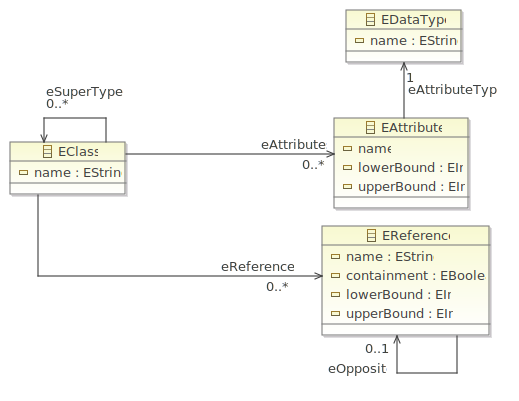
\includegraphics[height=10cm]{include/figures/Ecore}
	\caption{An illustrative core part of Ecore, the metamodeling language of EMF}
	\label{fig:Ecore}
\end{figure}

\Cref{fig:Ecore} shows only a small fraction of the metamodel, as there is many more classes in the Ecore metamodel. The main classes are the following:
\begin{itemize}[topsep=0pt]
	\item \code{EAttribute} represents a named attribute literal, which also has a type.
	\item \code{EClass} represents a class, with optional attributes and optional references. To support inheritance, a class can refer to a number of supertype classes.
	\item \code{EDataType} is used to represent simple data types that are treated as atomic (their internal structure is not modeled). Data types are identified by their name.
	\item \code{EReference} represents a unidirectional association between \code{EClass}es and is identified by a name. It is also possible to mark a reference as a containment that represents composition relation between elements. A bidirectional association should be modeled as two \code{EReference} instances mutually connected via their opposite references.
\end{itemize}

An Ecore model has a root object, representing the whole model. The children of this root object are packages, and the children of those are classes.

More detailed illustrations of the metamodel can be found in the EMF Documentation~\cite{ecore}.


\subsubsection{VIATRA Query}
VIATRA is an event-driven and reactive model transformation platform. \textquote[\cite{viatra}]{The VIATRA framework supports the development of model transformations with specific focus on event-driven, reactive transformations and offers a language to define transformations and a reactive transformation engine to execute certain transformations upon changes in the underlying model. Furthermore, the underlying incremental query engine, originating from the EMF-IncQuery project is reusable in different scenarios not related to model transformations.}

VIATRA Query (formerly IncQuery) is an incremental query engine with its own graph pattern based query language to specify and execute model queries on EMF instance models or other data storage solutions.

Since the data model of my approach may change over time, an unstructured or semi-structured data storage suits it better. EMF would require the metamodel to be transformed each time it is changed. It is also not possible to shard large EMF models in and take advantage of a clustered environment.


\section{Visual Studio Code}
Visual Studio Code~\cite{vscode} is Microsoft's take on a lightweight, yet powerful Integrated Developer Environment (IDE) for modern programming languages. It is available for free for Windows, OS X and Linux. It comes with built-in support for JavaScript, TypeScript and has a growing ecosystem of extensions for other languages, theming, and developer support~\cite{vscode-extensions}.

Debugging is also made easy, as the editor can be attached to the running code and the developer can add break points, look at call stacks and evaluate statements with an interactive console. With the relatively small package, Git support comes built-in: reviewing changed lines, staging files, making commits can be made right in the IDE.

\subsection{IntelliSense}
Visual Studio Code's syntax highlighting and autocomplete system is called IntelliSense, that also provides better completition based on variable types, function definitions, and imported modules. IntelliSense provides syntactical features like \emph{format on type}, \emph{outlining}; and also language service features like \emph{peek}, \emph{go to definition}, \emph{find all references} and \emph{rename symbol}.

To make these smarter functions possible, JavaScript service relies upon the TypeScript language service to handle JavaScript source code. It uses the same type inference system as TypeScript to determine the type of a value. (It recognises the \emph{``ES3-style''} class declaration.) Explicit JSDoc annotations can also be used, in case the type inference does not provide the desired type information. For major libraries it is also possible to download an import a type definition file.

\subsection{Extensions}
Visual Studio Code is built with extensions in mind. Extensions make it possible to add new languages, themes, debuggers, and to connect to additional services. The framework runs them in a separate process, ensuring they will not slow the editor down.

Every extension has the same model describe its contribution (how it is registered in the framework), activation (when it is loaded) and the same way to access the VS Code extension API. There are two special type of extensions: language servers and debuggers, which have their own additional protocols.

Extensions are the building blocks of VS Code. When activated, every extension runs in a shared host process, separate from the IDE. This ensures that the IDE itself can remain responsive even if an extension is resource-heavy or not well-written.

An extension is a package of source code, resources, and configuration files. They have support for:
\begin{itemize}[topsep=0pt]
  \item Activation -- it is possible to specify when an extension is loaded: when a specific file type exists in the workspace or is opened; or when a command (described in the configuration) is executed via the \emph{Command Palette} or the key combination.
  \item Editor -- the extension can read and manipulate the editor's content.
  \item Workspace -- the extension can access working files, modify the content of the status bar and show information messages (and more).
  \item Eventing -- it is also possible to subscribe and react to the life-cycle events of the editor such as: open, close, change events of the editor (and more).
  \item Evolved editing -- rich language support can be provided, including IntelliSense services, peek, hover and diagnostic (info, warning and error messages).
\end{itemize}

\paragraph{Language Servers} For high cost IO or CPU intensive tasks.
Language server framework and sample implementation helps developers create a dedicated process for resource-heavy language server applications. It is the better design choice if the extension may slow down other extensions while working. Its possibilities are limited, as custom communication between the client extension and the language server needs modification in the underlying communication protocol handler.

\paragraph{Debuggers} Connecting an external debugger written for any language to VS Code is also possible through the VS Code Debug protocol.
